\chapter{Risultati}%Caratterizzazione DDS su HPC
% Visti i diversi risultati si può dire che è meglio usare i topic per* le partizioni per *
% etc etc

Nella sezione corrente, si riportano tutti i risultati rilevanti ottenuti durante la fase di testing, stilando un possibile modello di use-case utile alle finalità di Power Management.
\section{Discovery centralizzata contro distribuita}
Come previsto, nella fase di discovery un numero elevato di entità genera una quantità di operazioni da svolgere che cresce in modo esponenziale. In questo caso sono stati usati tutti i core di due nodi, con un totale di 96 entità.
Già nel primo grafico è possibile notare un distacco tra i due approcci, con sole 30 unità \ref{fig:test0pack}. Nelle figure dei cicli \ref{fig:test0cicl} e delle istruzioni \ref{fig:test0_instr} viene confermato l'andamento non lineare.

\begin{figure}[H]
    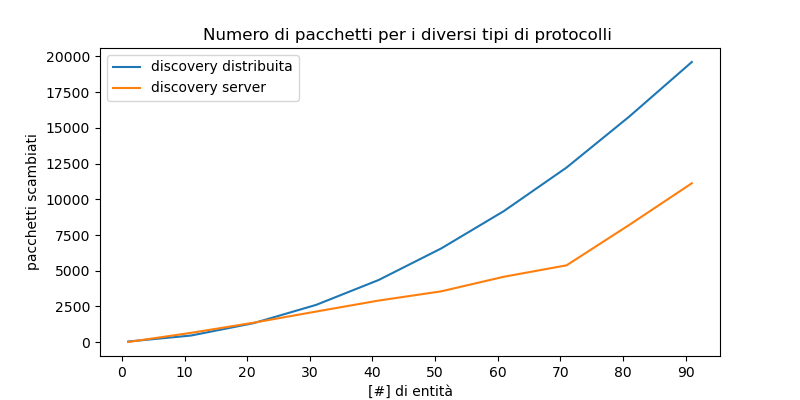
\includegraphics[width=\textwidth]{./results/test0_packet.png} 
    \caption{Numero di pacchetti scambiati durante la discovery all'aumentare di entità} %TODO: caption
    \label{fig:test0pack}
\end{figure}
\begin{figure}[H]
    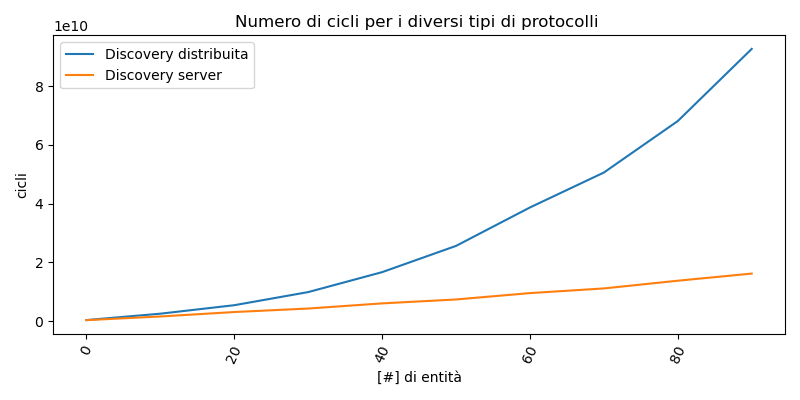
\includegraphics[width=\textwidth]{./results/test0_cicli.png} 
    \caption{Numero di cicli durante la discovery all'aumentare di entità nelle diverse opzioni} %TODO: caption
    \label{fig:test0cicl}
\end{figure}
\begin{figure}[H]
    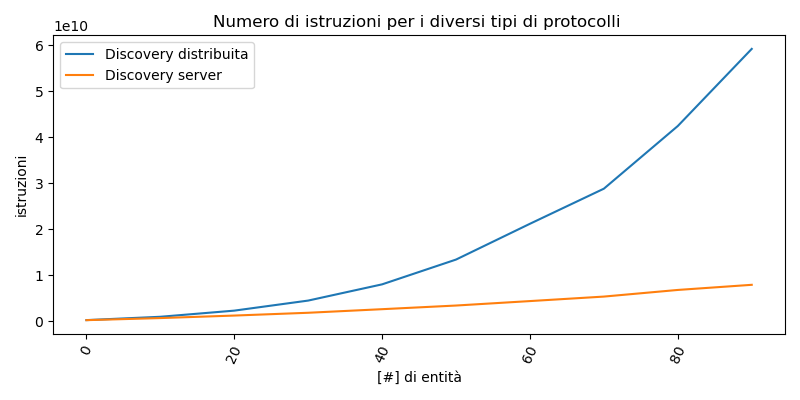
\includegraphics[width=\textwidth]{./results/test0_istruzioni.png} 
    \caption{Numero di cicli durante la discovery all'aumentare di entità nelle diverse opzioni} %TODO: caption
    \label{fig:test0_instr}
\end{figure}
In un caso reale serve valutare in primo luogo il numero di entità in un determinato dominio, e successivamente i costi-benefici di ogni implementazione considerando anche l'impatto che si può avere nel caso di fallimento del server (nonostante sia possibile avere un server di backup che viene automaticamente attivato, nel caso il primo fallisse)

\section{Impatto del numero di sub iscritti ad un topic}
Visto lo schema \ref{fig:uml} si può capire, che il numero di subscriber presenti in un dominio ed iscritti ad un topic, comporta un overhead di comunicazione che va ad influenzare sia i tempi, che cicli e istruzioni impiegate nella singola \emph{publish} come viene dimostrato nella figura \ref{fig:test3_overhead} e \ref{fig:test3_latenza}. L'effetto è particolarmente pronunciato anche in protocolli come \emph{UDP} che non dovrebbero possedere concetti di connessione. Questo potrebbe essere dovuto al costo di inizializzazione ed invio dei messaggi, ad indirizzi di rete diversi.
\begin{figure}[H]
    \centering
    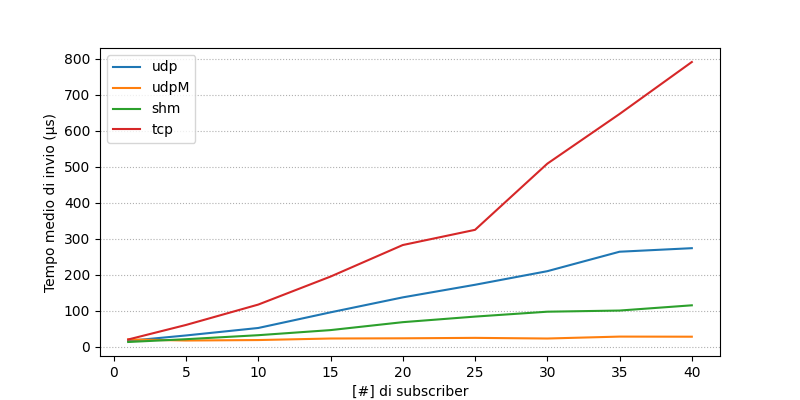
\includegraphics[width=\textwidth]{./results/test3_sending_multiplesub.png} %TODO, sqeunce is an error
    \caption{overhead sulla publish all'aumentare dei subscriber}
    \label{fig:test3_overhead}
\end{figure}
\begin{figure}[H]
    \centering
    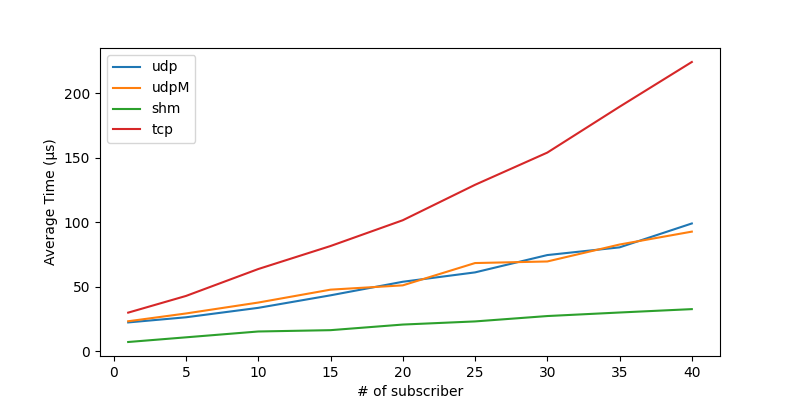
\includegraphics[width=\textwidth]{./results/test3_sendingreceiving_multiplesub.png} 
    \caption{latenza di ricezione all'aumentare dei subscriber}
    \label{fig:test3_latenza}
\end{figure}

Ovviamente l'impatto è poco significativo in quei protocolli che applicano strutture di \gls{multicasting} come udp-Multicast e Shared-Memory, che verranno 

\begin{figure}[H]
        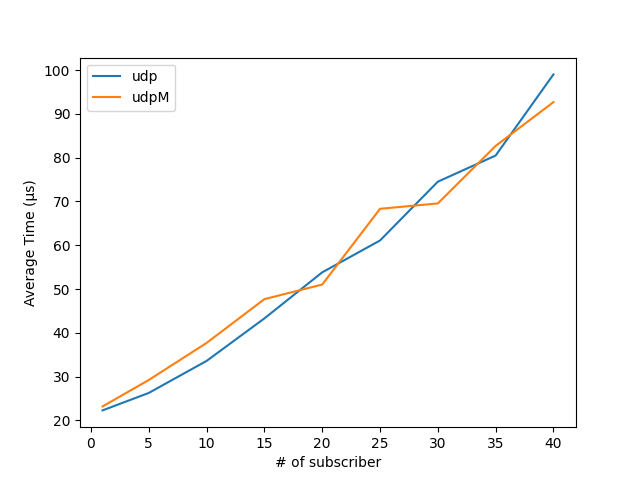
\includegraphics[width=\textwidth]{./results/test3_udpvsudpM.png} 
        \caption{} %TODO: caption
        \label{}
\end{figure}

Da questo si può concludere che sia il publisher che subscriber risentono della presenza di molteplici \emph{dds-partecipant} in ascolto su un topic. Questo problema è migliorato nel caso vengano utilizzati protocolli che si basano su multicast. 

\section{Primo messaggio}
E' stato notato con tutti i protocolli utilizzati un ritardo, di un ordine di grandezza superiore, che riguarda esclusivamente il primo messaggio. Tuttavia, non è stato chiarito il motivo di questo \gls{overhead}, presente anche in comunicazioni locali\footnote{comunicazioni effettuati in localhost o in shared memory}. Anche se non dimostrato una delle possibili motivazioni potrebbe essere la necessità di allocare memoria durante la prima fase di comunicazione, da entrambi gli attori (potenzialmente amplificato nel caso \ref{fig:rtt_uml}). 
\begin{figure}[H]
    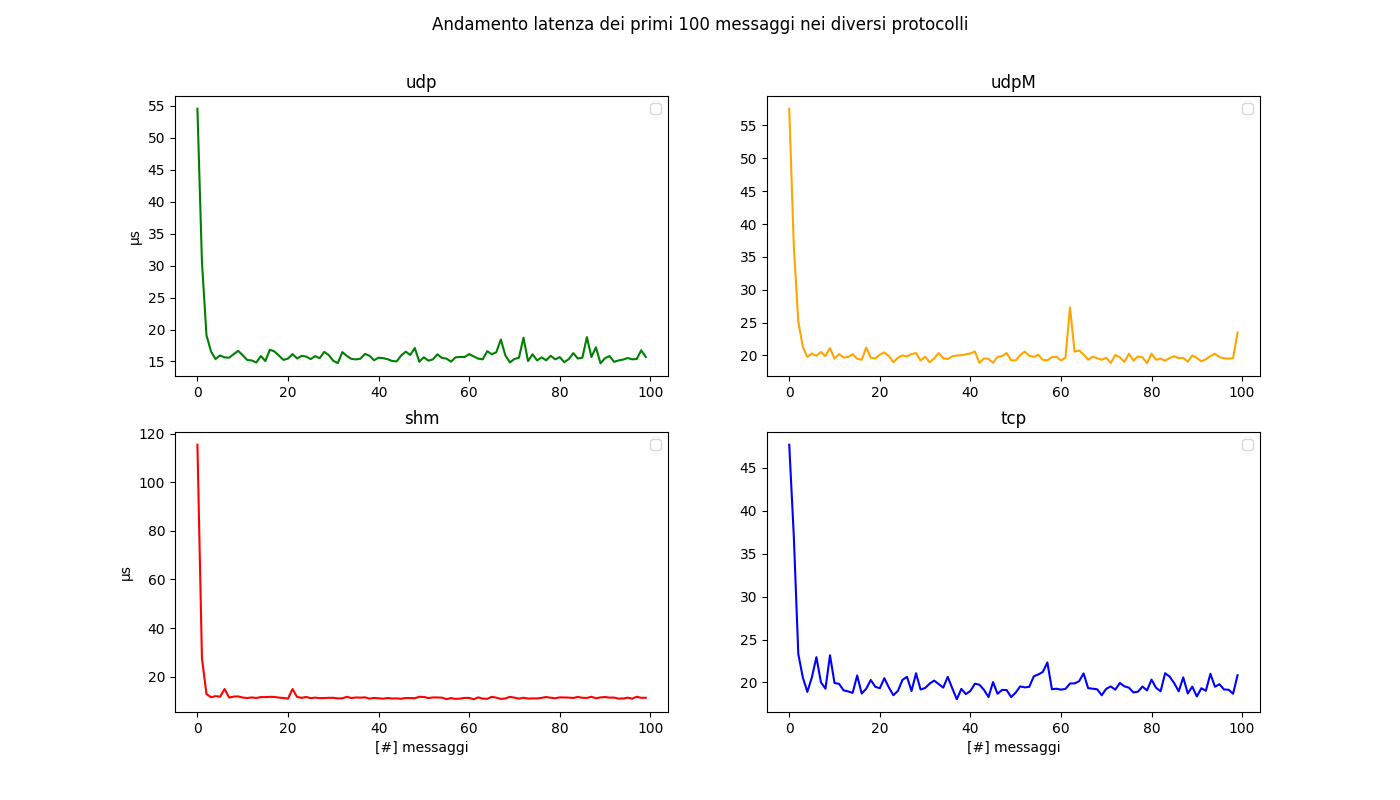
\includegraphics[width=\textwidth]{./results/errortest.png} 
    \caption{} %TODO: caption
    \label{}
\end{figure}
Data la complessità necessaria per andare così a fondo nel problema, non è stato approfondito ulteriormente.

\section{Protocolli di comunicazione}
Visti gli schemi \ref{fig:schema_global} è prevedibile che in un vero Power Stack, siano predilette le comunicazioni non locali. In merito a ciò, nonostante ci siano di mezzo molti più livelli per comunicare con udp e tcp, i risultati trovati sono stati decisamente interessanti e non così lontani dal più veloce \emph{Shared Memory}.

\begin{figure}[H]
    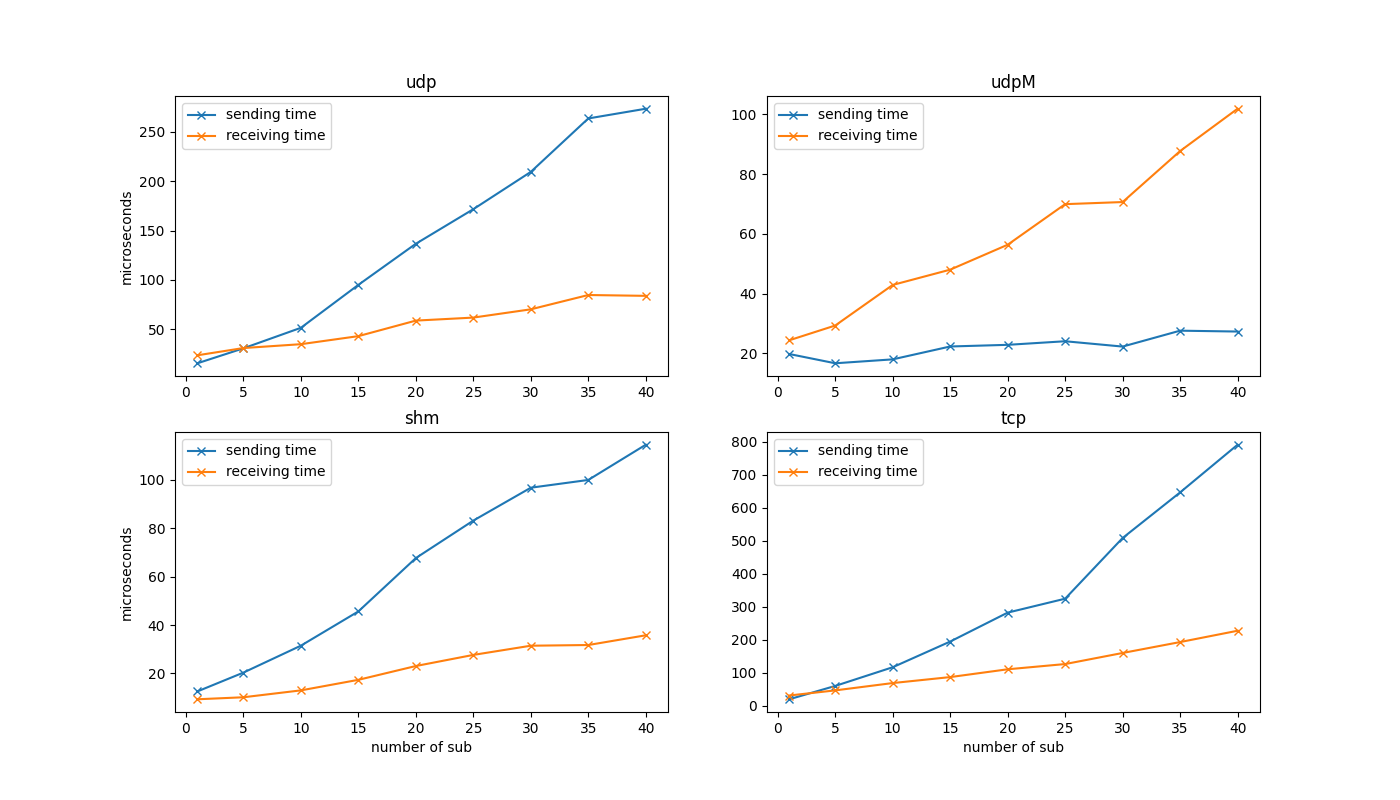
\includegraphics[width=\textwidth]{./results/test3_different_protocol_send_receive.png} 
        \caption{differenza tra solo publish e publish-subscribe per ogni protocollo}%TODO Da sistemare immagine, sending receivin non va bene, label sbagliate etc
        \label{fig:test3_different_protocols}
\end{figure}


\begin{figure}[H]
    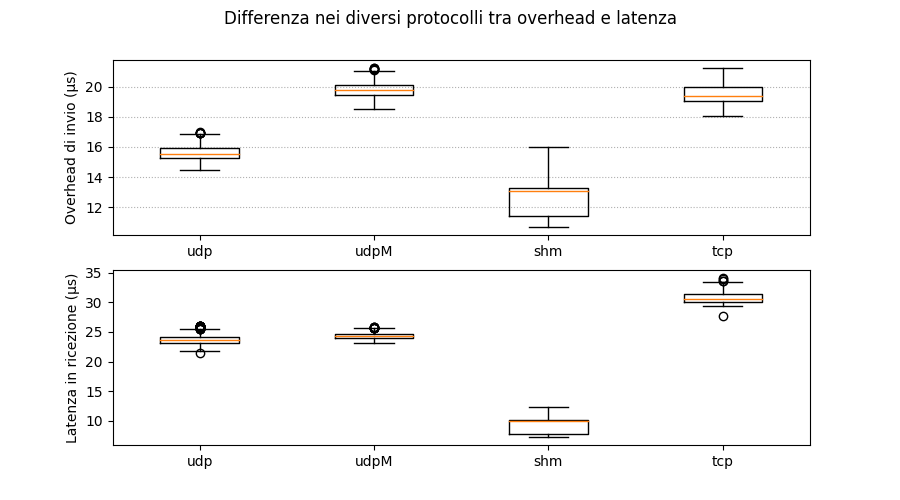
\includegraphics[width=\textwidth]{./results/test1_box_sr_1p1s.png} 
        \caption{diagramma a scatola nei vari protocolli di comunicazione con un publisher e un subscriber}
        \label{fig:test1sdbox}
\end{figure}

\begin{figure}[H]
    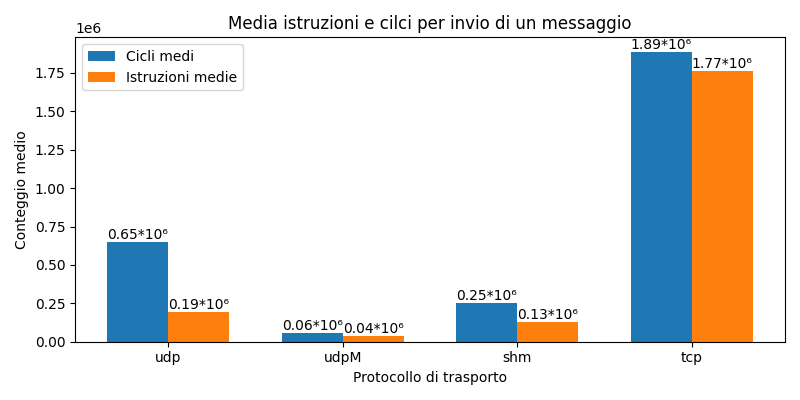
\includegraphics[width=\textwidth]{./results/test1_cyclinstr.png} 
        \caption{Conteggio cicli e istruzioni per ogni protocollo}
        \label{fig:test3_different_protocols}
\end{figure}
E' quindi preferibile, ove possibile, usare \emph{Shared Memory} sia per prestazioni, che per evitare di saturare la rete. In secondo luogo, se in presenza di diversi subscriber, per non caricare il publisher usare \emph{UDP Multicast}. E infine utilizzare \emph{TCP} solo dove vi è necessità di connessione, visto le notevoli latenze si in scrittura che in lettura. In tutti gli altri casi, dove non si è in locale, e dove il numero di subscriber non supera qualche decina, risulta più che adeguato \emph{UDP}.

\section{Domini, Partizioni e Wildcards}
Nei test effettuati con topic e partizioni, non sono state notate differenze degne di nota in termini di performance nell'usare uno strumento piuttosto che un altro (\ref{fig:test2parttopicdomain}). Lo sono stati invece tra questi ultimi e i Domini. Tuttavia i domini non offrono alcun tipo di flessibilità e richiede il riavvio dei \emph{dds-partecipant} nel caso si necessiti di un qualsiasi cambiamento. Per questo è consigliato utilizzo di domini diversi, solo tra entità che non hanno necessità di comunicare, e che anzi, magari anche per motivi di sicurezza devono stare isolati. 


\begin{figure}[H]
    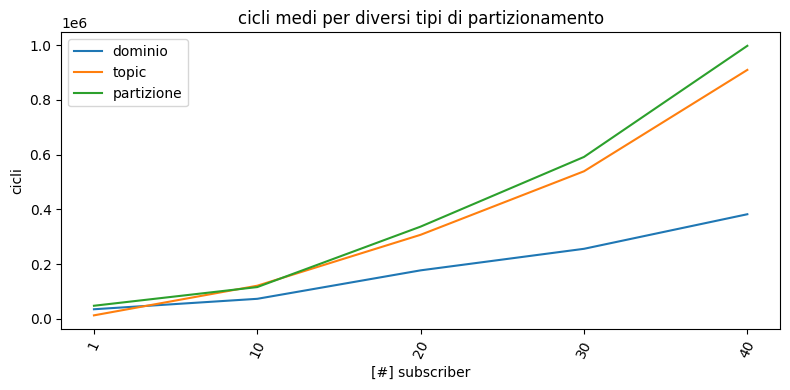
\includegraphics[width=\textwidth]{./results/test2_cicli_partvstopicvsdomaain.png} 
        \caption{Peso in termini di cicli nell'usare partizioni topic e domini}
        \label{fig:test2parttopicdomain}
\end{figure}

Per quanto riguarda entità che necessitano di gerarchie, è conveniente usare le partizioni con le Wildcards visto che non hanno un peso significativo \ref{fig:test2wildcards}. Infine lasciando i topic come mezzo di partizionamento, per il tipo di dati, e il tipo di istruzioni da utilizzare.

\begin{figure}[H]
    \centering
    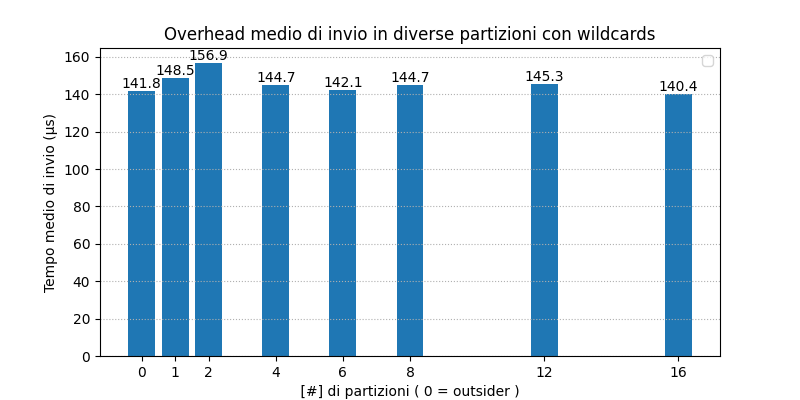
\includegraphics[width=\textwidth]{./results/test2_wildcards.png}
    \caption{La differenza tra dummy, 1 partizione o 16 partizioni non ha particolari costi in termini di invio con utilizzo di wildcards}
        \label{fig:test2wildcards}
\end{figure}



\section{Throughput}
L'ultimo test è stato utile a comprendere tutte le potenzialità di questo strumento più che creare un modello di utilizzo. Infatti come si può vedere dai seguenti grafici, i numeri di KByte (\ref{fig:throughput_combined}) che è possibile inviare ogni secondo da un publisher ad un subscriber supera il MB/s, e permettendo comunicazione di diverse decine di Hz (\ref{fig:throughput_combined}). Inoltre questo valore raggiunge numeri ancora più elevati qualora si usassero comunicazioni multicast, come notabile in figura \ref{fig:throughput_increasing}.
\begin{figure}[H]
    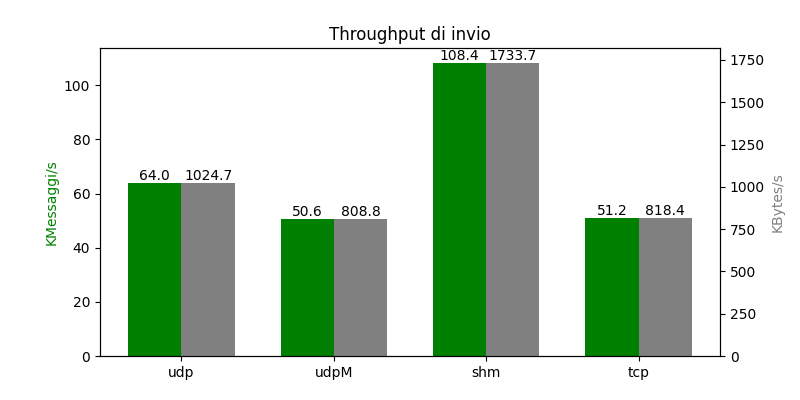
\includegraphics[width=\textwidth]{./results/test3_throughput_combined.png} 
        \caption{throughput di invio da parte di un singolo attore}
        \label{fig:throughput_combined}
\end{figure}
Sull'asse delle Y, a sinistra, vengono mostrati in verde i il valore di KMessaggi/s\footnote{1000 Messaggi al secondo} raggiungibili dai vari protocolli di comunicazione, mentre in grigio, a sinistra i KByte/s.

% \begin{figure}[H]
%     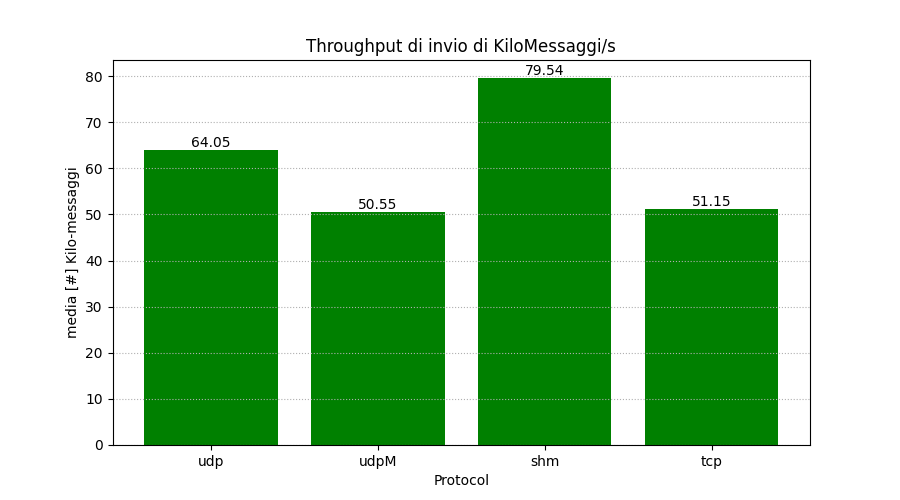
\includegraphics[width=\textwidth]{./results/test3_throughput_m.png} 
%         \caption{throughput di invio da parte di un singolo attore in messaggi} %TODO: caption
%         \label{fig:throughput_msg}
% \end{figure}


\begin{figure}[H]
    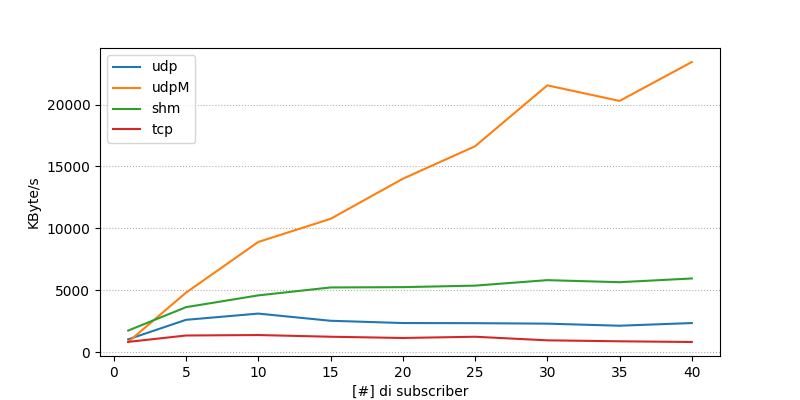
\includegraphics[width=\textwidth]{./results/test3_graph_throughput.png} 
    \caption{throughput a crescenti numeri di subscribers} 
    \label{fig:throughput_increasing}
\end{figure}

